
\section{Spin density wave instability}
\label{Sec:Theo:SpinDensityWave}

\begin{figure}[htbp]
    \begin{center}
        \includegraphics[scale=0.8]{Chapter-Introduction/Figures/SpinFluctuationPairing/SpinFluctuationPairing}
        \caption{A schematic illustration of the mechanism of spin fluctuation mediated pairing. Two itinerant electrons (filled circles) are bound via exchange interactions, $J$, to electrons in the electron gas coupled by an antiferromagnetic spin fluctuation (large dotted line) over a wavevector $q$. Adapted from ref.~\cite{Cox1995}}
        \label{Fig:Intro:SpinFluctuationPairing}
    \end{center}
\end{figure}

The schematic mechanism of spin fluctuation mediated pairing is illustrated in figure~\ref{Fig:Intro:SpinFluctuationPairing}. The first itinerant electron, $e_1$, couples to an electron in the background electronic continuum, $e_2$, which is subject to an antiferromagnetic fluctuation. They couple via the exchange interaction, $J$, and the spin of $e_2$ flips so that it is opposite to $e_1$. The spin flip propagates through the background electron gas to another electron, $e_3$, via the spin fluctuation interaction, which makes the location in close proximity favourable to an electron of opposite spin thus drawing in $e_4$ via the exchange interaction. The end result is a Cooper bound state of two itinerant electrons ($e_1$ and $e_4$) via an antiferromagnetic interaction in the background electron continuum.


Section~\ref{Sec:Intro:Nesting} discussed the possibility of high-$T_c$ pairing being due to fluctuations in close proximity to a \ac{SDW} state. Here we briefly describe the \ac{SDW} state and some of the theory behind it.

Broadly speaking a \ac{SDW} is a magnetic state just as ferromagnetism and antiferromagnetism are magnetic states. In its most general sense, a \ac{SDW} is a periodic modulation of magnetic spins in both space and time hence it being a `wave of spin density'. \ac{AFM} is actually a special case of a \ac{SDW} which does not vary in time, i.e. is static, and also varies spatially with the periodicity being some multiple of the real-space lattice vector, i.e. is commensurate with the lattice. Ferromagnetism can be thought of as a \ac{SDW} state with wavevector $\vect{q}=0$ i.e. it has no periodic variation and so is not really a `wave'.

Using the mean field \ac{HFA} the following expression gives the stability condition for the \ac{SDW} state~\cite{Moriya1985},
\begin{equation}
2I\chi_0(\vect{q}) > 1,
\end{equation}
where $I$ is the exchange energy between electron bands and $\chi_0$ is the Lindhard susceptibility. The greater the Lindhard susceptibility, the more stable the state.

\subsection{Lindhard susceptibility}
\label{Sec:Theo:Susceptibility}

The Lindhard susceptibility models the Stoner excitations (i.e. electron-hole scattering) of a nearly free electron system. To derive the Lindhard susceptibility, we begin with a Fermi liquid i.e. a Pauli excluded but otherwise non-interacting gas of free electrons. We calculate\footnote{Not presented here but pg 81 ff. of Dressel~\cite{Dressel2002} has a full derivation.} the first order perturbative linear response of this gas to a magnetic field given by $\vect{B}=\exp{(\vect{q}.\vect{r} - i\omega.t})$. The resulting equation is often quoted as,
\begin{equation}
    \chi_0(q, \omega) = \lim_{\delta \to 0} \sum_{k}\sum_{l,l^\prime}\frac{f(\epsilon_{k+q,l^\prime}) - f(\epsilon_{k,l})}{\epsilon_{k+q,l^\prime} - \epsilon_{k,l} - \hbar\omega - i\delta}D
    \label{Eqn:Intro:Lindhard}
\end{equation}
where,
\begin{equation}
    D = |\langle k+q,l^\prime|V|k,l \rangle|^2
\end{equation}
and is the matrix transition element for the scattering process. The numerator term contains two Fermi functions --- the same as equation~\ref{Eqn:Theo:FermiFunction} --- which ensure that the susceptibility is finite for states which scatter across the Fermi energy and zero if they do not - consequently, the Lindhard susceptibility models electron-hole scattering (Stoner excitations) in particular. The Fermi functions also smear the susceptibility dispersion as a function of temperature. The third term in the denominator corresponds to the excitation energy of the perturbing field with $\omega$ corresponding to the temporal frequency of the field. The final term in the denominator is an artefact of the adiabatic approximation used to calculate the perturbation with the completed approximation taking the limit of $\delta \to 0$. The first sum in the Lindhard function is over all $k$ states in the first \ac{BZ}, the second sum combines each energy band. The real and imaginary parts of equation~\ref{Eqn:Intro:Lindhard} are,
\begin{align}
\Real\{\chi_0(q, \omega)\} &= \lim_{\delta \to 0} \sum_{k}\sum_{l, l^\prime}\frac{(\epsilon_{k+q,l^\prime} - \epsilon_{k,l} - \hbar\omega) (f(\epsilon_{k+q,l^\prime}) - f(\epsilon_{k,l}))}{(\epsilon_{k+q,l^\prime} - \epsilon_{k,l} - \hbar\omega)^2 + \delta^2}D \\
\label{Eqn:Theo:ReLindhard}
\Imag\{\chi_0(q, \omega)\} &= \lim_{\delta \to 0} \sum_{k}\sum_{l, l^\prime}\frac{-\delta (f(\epsilon_{k+q,l^\prime}) - f(\epsilon_{k,l}))}{(\epsilon_{k+q,l^\prime} - \epsilon_{k,l} - \hbar\omega)^2 + \delta^2}D\\
\label{Eqn:Theo:ImLindhard}
\end{align}
respectively. The real part is important in the context of instabilities in metals, the imaginary part gives the resonance modes for bosonic excitations such as e.g. plasmons, spin density waves, charge density waves, phonons etc. of energy $\hbar\omega$.

The Lindhard function is a simple linear response for a particular static charge configuration. As soon as the charge configuration shifts due to the perturbing field the potential changes and so does the response. To compensate we consider the perturbing field to be adjusted by considering an additional induced field due to the changing charge along with the perturbing field and calculate the linear response in terms of that new combined field. This new form is the `first renormalisation'. This is still not perfect however since now the charge density changes again in a different way due to this new combined potential and so a second induced potential has to be considered giving the `second renormalisation' and so-on. This process of renormalisation forms the basis of linear response theory. In practice the \ac{RPA}\footnote{So called because it is considered that the charge densities in the higher renormalisations are from electron wavefunctions which have randomly shifted phases and so cancel each other out.} is generally invoked where corrections beyond the first renormalisation are ignored. The \ac{RPA} response of the Lindhard susceptibility is as follows,
\begin{equation}
    \chi(\vect{q},\omega) = \frac{\chi_0(\vect{q}, \omega)}{1 - \frac{4\pi e^2}{q^2} \chi_0(\vect{q}, \omega)}
\end{equation}

The renormalised susceptibility is not therefore necessarily at a maximum when the Lindhard, linear response, susceptibility becomes singular, rather the renormalised \ac{RPA} susceptibility tends to $\pm1$. Peaks in the Lindhard susceptibility function correspond to scattering of states which cross the Fermi energy yet remain close to the Fermi energy.  We can derive this function by modelling an oscillatory perturbing field on a system. To solve to get an expression for the second order perturbation, we make the adiabatic limit approximation (i.e. the perturbing potential is gradually increase from zero at $t=\infty$ to $v$ at $t=0$).

Although knowledge of the susceptibility is useful to model, for example, neutron scattering measurements, for our purposes we will use it as an indicator of possible \ac{SDW} instability vectors in our example materials. For this reason we make the assumption that the transition matrix elements are unity. This assumption greatly simplifies the calculations at the cost of some structure and as such should be borne in mind that the results are somewhat broad and qualitative.


\subsection{Notes on practical calculation}

Taking the limits of $\delta \to 0$ of equation~\ref{Eqn:Theo:ImLindhard} which is effectively an ever narrowing Lorentzian distribution, results in an expression for the imaginary part of Lindhard susceptibility, $\Imag(\chi_0)\propto \delta(\epsilon_{k+q,l^\prime} - \epsilon{k,l} - \hbar\omega)$ where $\delta$ here is the Dirac delta function. In a calculation on a continuous energy dispersion, this results in resonances at excitations which match the difference in energies between states. However, in this thesis, the energy dispersions used to determine nesting conditions are not continuous and instead are based on discrete energies obtained from \ac{DFT} calculations. As such $\delta$ will have to remain finite in order to broaden the delta function into a Lorentzian with width comparable to the energy differences between the discrete points -- the net result of this will be loss of some fine structure.

Secondly, only bands that lie close to the Fermi energy contribute significantly to the susceptibility. Since the calculations are computationally costly, only bands which are close (within the adiabatic or temperature broadening) to the Fermi energy are input into the calculations.
